% \documentclass[a4paper, technote, draft, compsoc]{IEEEtran}
\documentclass[a4paper, technote,compsoc]{IEEEtran}
%\documentclass[a4paper]{article}

\usepackage[toc,page,titletoc]{appendix}
\usepackage[T1]{fontenc}    % use 8-bit T1 fonts
\usepackage[utf8]{inputenc} % allow utf-8 input
\usepackage{amsmath}
% \usepackage{hyperref}
\usepackage{amssymb}
\usepackage{booktabs}
\usepackage{float}  % used to fix location of images i.e.\begin{figure}[H]
\usepackage{graphicx}  %needed to include png, eps figures
\usepackage{mwe}
\usepackage{url} % correct bad hyphenation here
\usepackage[dvipsnames]{xcolor}
% \usepackage{todonotes}
\usepackage{xr}
\usepackage{subfiles}
\usepackage{physics}
\usepackage{epigraph}

\usepackage{todonotes,tocloft,xpatch,hyperref}
\hypersetup{
    colorlinks,
    linkcolor={red!50!black},
    citecolor={blue!50!black},
    urlcolor={blue!80!black}
}

% This is based on classicthesis chapter definition
\let\oldsec=\section
\renewcommand*{\section}{\secdef{\Sec}{\SecS}}
\newcommand\SecS[1]{\oldsec*{#1}}%
\newcommand\Sec[2][]{\oldsec[\texorpdfstring{#1}{#1}]{#2}}%

% https://tex.stackexchange.com/a/61267/11984
\makeatletter
\xapptocmd{\Sec}{\addtocontents{tdo}{\protect\todoline{\thesection}{#1}{}}}{}{}
\newcommand{\todoline}[1]{\@ifnextchar\Endoftdo{}{\@todoline{#1}}}
\newcommand{\@todoline}[3]{%
  \@ifnextchar\todoline
    {}
    {\contentsline{section}{\numberline{#1}#2}{#3}{}{}}%
}
\let\l@todo\l@subsection
\newcommand{\Endoftdo}{}

\AtEndDocument{\addtocontents{tdo}{\string\Endoftdo}}
\makeatother


\externaldocument[M-]{main}

\usepackage[style=ieee]{biblatex}
\bibliography{xampl}
% \usepackage[backend=biber,style=ieee]{biblatex} 
\bibliography{bibliography.bib} %your file created using JabRef

% https://tex.stackexchange.com/questions/246/when-should-i-use-input-vs-include
% \newcommand{\N}{\mathbb{N}}
\newcommand{\Z}{\mathbb{Z}}
\newcommand{\Q}{\mathbb{Q}}

\newcommand{\R}{\mathbb{R}}
\newcommand{\RR}{\mathbb{R}^2}
\newcommand{\RRR}{\mathbb{R}^3}

\renewcommand{\Pmu}{\mathcal{P}}
\renewcommand{\P}{\mathbb{P}}

\newcommand{\delt}{\Delta t}
\newcommand{\utk}{{\widetilde u}^k}
\newcommand{\ut}[1]{{\widetilde u}^{#1}}
\newcommand{\rhog}{\text{\boldmath{$\rho$}}}
\renewcommand{\eps}{\varepsilon}

\DeclareMathOperator{\sspn}{span}
\newcommand{\spn}[1]{\sspn\left(#1\right)}
\newcommand{\mytodo}[1]{\todo[inline, color=green!20, inlinewidth=\columnwidth]{#1}}

\begin{document}

\onecolumn

% paper title
\title{
    \large{(Hyper) Reduced Order Models For Moving Meshes}
    \\[5mm] Literature Review \& Research Project 
    }

% author names 
\author{Enrique Millán Valbuena \\ \normalsize{463 426 8}}% <-this % stops a space
        
% The report headers
\markboth{M. Sc. Aerospace Engineering, TU Delft}%do not delete next lines
{Shell \MakeLowercase{\textit{et al.}}: Bare Demo of IEEEtran.cls for IEEE Journals}

% make the title area
\maketitle

\begin{IEEEkeywords}
    \centering
    Finite Elements, Galerkin, Reduced Order Models, 
    Moving Piston, Deforming Mesh, ALE, 
    (M)DEIM, POD, 
    Model Truncation
\end{IEEEkeywords}

\setcounter{tocdepth}{2}
\tableofcontents

\twocolumn

\section{Research Project}
This thesis focuses in the efficient numerical solution of parametrized unsteady PDEs with moving meshes.

Parametrized PDEs can be numerically solved with the finite element method (FEM), 
which leads to an algebraic system of equations whose solution 
can be computationally expensive to obtain, 
especially for complex geometries or elaborate models.
One refers to this FEM model as the \textit{Full Order Model}~(FOM),
\begin{equation}
   \frac{du_h}{dt} + A_h\left(t;\mu\right) u_h = f_h\left(t;\mu\right).
\end{equation}
When the problem is unsteady, that is, 
when the differential operators contain terms that change in time,
or the mesh moves in time (effectively changing the integrals of the weak form),
the algebraic operators need to be reassembled for each timestep.

When this is the case, many-query procedures and access to field values or 
calculated outputs for different parameter values $\mu$ can become cumbersome, 
or even infeasible due to computational costs, both in time and memory.
To circumvent the efficiency issues, one can build a \textit{Reduced Order Model}~(ROM), 
whose solution is fast in time and light in storage.
This ROM is based in ad-hoc empirical basis functions to represent the solution, 
whose support typically spans the whole domain. 

However, due to the change in time of the operators, 
using a standalone reduced basis to represent the solution
is not enough to remove all the overheads of the FEM model.
The operators still need to be assembled 
and projected in the reduced space for each timestep.
The reduced basis of the solution does shrunk the overall dimension of the system,
but it cannot remove the overhead derived from the inevitable change in the operators.
We would state to have an \textit{offline-online coupling},
since information from the FOM is required to assemble the ROM.
To overcome this issue, a system approximation technique is introduced.
We then talk about an \textit{Hyper Reduced Order Model}~(HROM).

\subsection{Outline of the Reduction Process}
The construction of the ROM has mainly two stages:
\begin{itemize}
   \item Offline stage: construction of the ROM ingredients.
   \item Online stage: assembly of the ROM to solve the PDE for unseen parametrizations.
\end{itemize}

During the offline stage, the costly algebraic problem is solved for a subset of the parameter space.
Snapshots of the matrices, vectors and solutions are stored and processed via algebraic reduction algorithms, 
in order to obtain a reduced basis for each of them.

An example of reduction algorithms would be the Discrete Empirical Interpolation Method (DEIM) 
and its matrix version (MDEIM).
These reduction algorithms need to rely on a procedure to construct the basis, 
in our case we will use the Proper Orthogonal Decomposition (POD). 

The offline stage scales with the dimension of the Full Order Model, $N_h$, 
which is governed by the number of nodes in the mesh and the polynomial degree for the FEM basis.
Once the offline stage is over, a basis for each operator of the algebraic problem has been produced, 
of representative\footnote{
   The reduction of each operator might have required a different number of basis elements, 
   but they should be all of the same order of magnitude $N \ll N_h$ or smaller for the reduction process to be a success.}
size~$N \ll N_h$.
A projection matrix $\mathbb{V}$ is derived from the solution reduced basis, 
\begin{equation}
   \mathbb{V} \in \mathbb{R}^{N_h \,\text{x}\, N}.
\end{equation} 
This matrix will be used to project once and for all 
the algebraic operator reduced basis elements, 
our HROM building blocks.
The reduced bases for the solution and the algebraic operators 
are then used during the online stage, 
where for unseen parameters a small algebraic system is built and solved,
\begin{equation}
   \frac{du_N}{dt} + A_N\left(t;\mu\right) u_N = f_N\left(t;\mu\right).
\end{equation}
At this stage, it is paramount that the assembly of the operators\footnote{
   We shall overload notation and refer to \textit{the operator} for both the matrices and the functionals,
   unless explicit distinction is required.
} 
is independent of the original problem size $N_h$.
We state to have a perfect \textit{offline-online decoupling}.

Once the reduced problem has been solved, the solution can be projected back to the original physical mesh,
\begin{equation}
   u_h = \mathbb{V} u_N.
\end{equation}
Following these steps, access to field values or calculated outputs can be obtained lightly, 
provided the overall procedure is \textit{certified}: 
to prove in the online stage that the solution is sufficiently close 
to what it would have been if the actual FOM had been assembled and solved.

All the above is presented graphically in Figure~\ref{fig:overview_graph}.

\subsection{System Approximation}
An essential ingredient to achieve a perfect \mbox{offline-online} decoupling
is what we call an \textit{
   affine decomposition} 
of the algebraic operators.
Simply put, it is to say that we can achieve a linear separation 
in the parameter, time, and spatial domains 
(the latter represented by the algebraic basis elements), 
\begin{equation}
   A_h\left(t;\mu\right) = \sum_{q=1}^{Q} \Theta_{q}(t;\mu) A_{h,q},
\end{equation}
where~$A_{h,q}$ are constant matrices referred to as the collateral basis,
and~$\Theta_{q}(t;\mu) \in \mathbb{R}$ are scalar values. 

The easiest example one could come up with of an affine decomposition is the one present 
in the heat diffusion problem with two different but uniform diffusion parameters $k_q$ across the domain.
The affine decomposition would look like
\begin{equation}
   A_h\left(t;k_1, k_2\right) = k_{1} A_{h,1} + k_{2} A_{h,2},
\end{equation}
where each matrix $A_{h,q}$ would represent the diffusion operator with support over the subdomain associated with each parameter. 
For this simple example, the affine decomposition is present naturally within the PDE structure, 
but this will not always be the case, specially when nonlinearities are present. 

However, nowadays it is absolutely possible to obtain an automatic ad-hoc affine decomposition 
for any operator thanks to grounded algorithms and procedures, like DEIM and MDEIM.
This key fact will allows us to achieve a perfect split between the offline and the online stage, 
as it will allow us to assemble our ROM operators without having to assemble at any point the complete FOM operator. 

\subsubsection{Nonlinear Term Reduction}
The reduction of a nonlinear term can be achieved 
with the same MDEIM technique as the one used for linear operators.

The only difference is that the coefficient functions~$\Theta_{q}$ from 
the affine decomposition depend on the solution values too,
\begin{equation}
   A_h\left(t;\mu\right, u) = \sum_{q=1}^{Q} \Theta_{q}(t;\mu, u) A_{h,q}.
\end{equation}
Nevertheless, this fact does not necessarily break the convergence and approximation 
properties derived for MDEIM,
so we expect to use it successfully.   

% Ideally, 
%% Research objectives
% Useful: benefit of your research to the problem. 
% Realistic: contribute to the solution of the problem.
% Feasible: time scheduled and capabilities and resources.
% Clear: be precise in the contribution to the problem.
% Informative: rough idea of knowledge generated towards a solution.

% The research objective is (a) by (b).
% (a) The contribution of the research project to the solution of the problem.
% (b) description of the way the contribution will be provided. 

\subsubsection{Implicit \textit{Nonlinearities}}
A nonlinearity can be seen essentially as a characteristic that prevents a linear separation.
Despite the apparent linear character of an algebraic equation, 
from the point of view of the affine decomposition, 
it could potentially hide a nonlinearity.

The introduction of the time variable~$t$~in the shape of the mesh makes it so
that the operators change at each time step during the integration loop.
Additionally, since the domain geometry will depend on some parameter values too, 
one cannot explicitly write the affine decomposition of the operators in a closed form.
This is implicitly collected by the Jacobian,
the transformation that maps integrals over moving meshes 
to one over a reference fixed mesh.

Another type of nonlinearity would be a term whose integrand contained 
a nonlinear function applied over the $u$ field,
or interactions of the solution with its own derivatives.
% These kind of non-linearities are common in mathematical modelling, 
% but shall keep out of the scope of this work to keep a narrow focus. 
% The non-linearity of the basic operators will give us enough work already.

\subsection{Kick-off Point}
The (M)DEIM reduction technique have been successfully used with domains
whose boundary is parametrized, but whose mesh remained fixed in time \cite{Santo_Manzoni_2019}. 

We aim at extending these results by introducing a moving mesh in time,
thus allowing us to obtain an hyper reduced order model which can tackle 
more complex \mbox{real-life} problems.
The additional complexities introduced by the moving mesh are the introduction 
of the Arbitrary Eulerian Lagrangian formulation (ALE), 
and the increase in the number of operator snapshots to be collected during the offline stage.  

\onecolumn
\begin{figure}[h]
   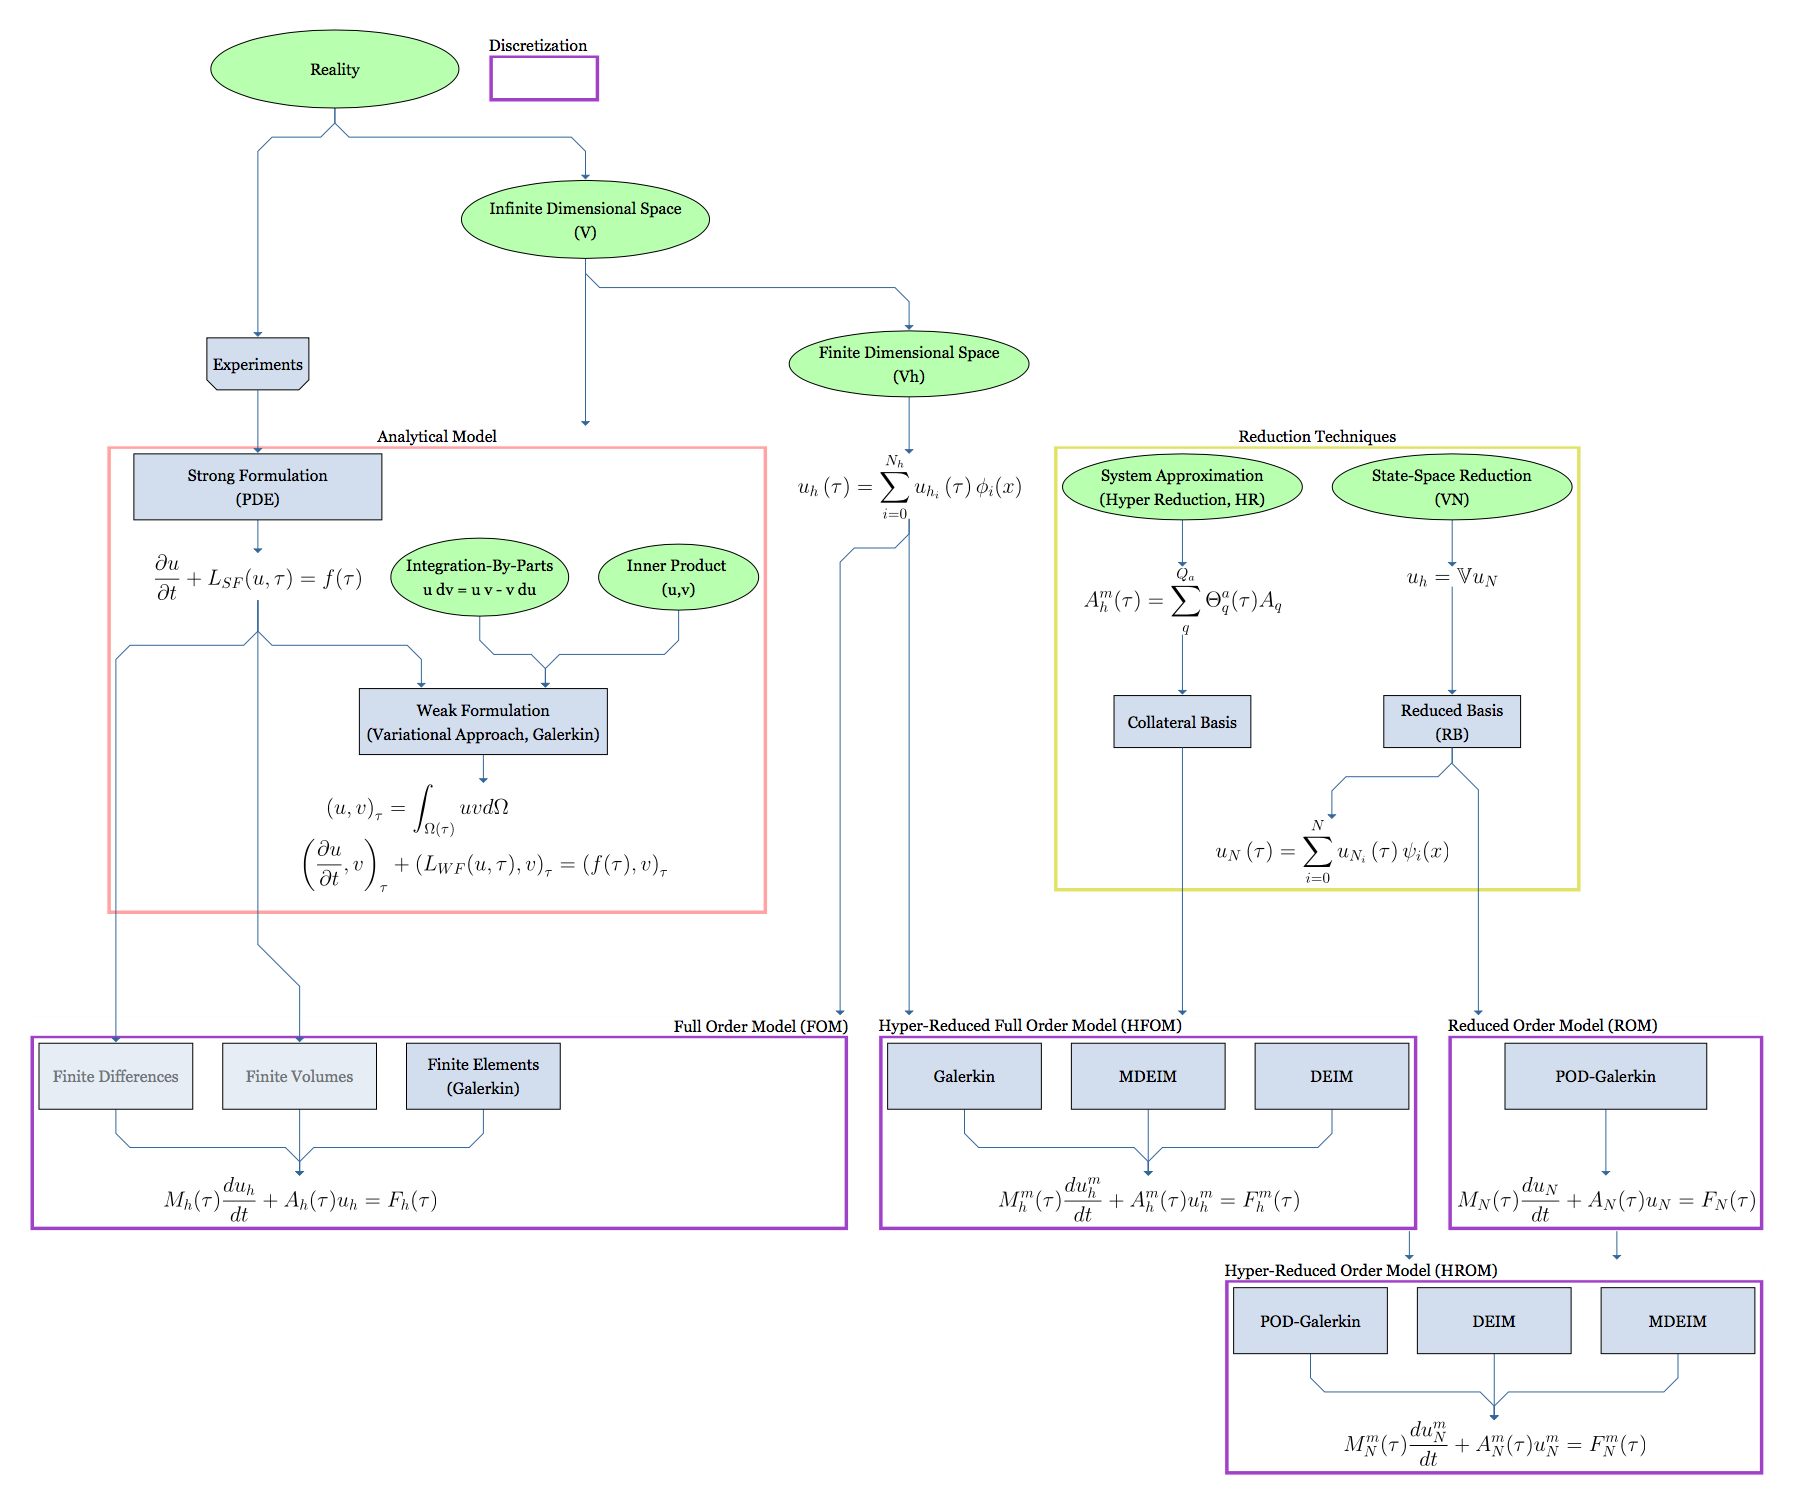
\includegraphics[width=\columnwidth]{graphs/From-Reality-To-ROM.png}
   \caption{Building blocks of the transition from reality to discrete 
   reduced order modeling.
   On the left side we present the traditional finite element course: 
   from the observation of reality a parametrized PDE model is derived 
   (infinite dimensional space, unknown analytical solution).
   The paremeters allow the model to capture a range of 
   boundary conditions, geometries,
   and term-domination effects, 
   all of them driven by the same physics.
   % 
   This model can be cast into a weak form and 
   solved numerically via the Galerkin projection 
   (finite dimensional space, Lagrangian piecewise solution).
   The finite element method is a robust and well-established technique
   for the solution of parametrized PDEs.
   However, for three-dimensional domains, 
   or complex modelling terms, the algebraic operators involved (vectors and matrices) 
   can become computationally expensive to assemble and solve,
   especially for unsteady problems with moving meshes.
   % 
   On the right side, we present two reduction techniques introduced 
   to increase the efficiency of the numerical solution:
   the construction of a \textit{reduced basis} (RB), also known as state-space reduction;
   and the determination of a collateral basis for 
   the algebraic finite element operators, known as \textit{system approximation}.
   The reduced basis is used in substitution of the Lagrangian piecewise functions,
   the collateral basis is used to skip the assembly 
   of all the entries of each algebraic operator.
   % 
   All in all, the simultaneous use of these two reduction techniques 
   leads to an algebraic hyper-reduced order model,
   cheaper to assemble and solve than the traditional finite element problem;
   and for problems with time-dependent matrices,
   even cheaper than assembling the operators and projecting them
   unto the reduced basis for each timestep.}
   \label{fig:overview_graph}
 \end{figure}
 \twocolumn

\section{Literature Review}
%% Lab Report for EEET2493_labreport_template.tex
%% V1.0
%% 2019/01/16
%% This is the template for a Lab report following an IEEE paper. Modified by Francisco Tovar after Michael Sheel original document.


%% This is a skeleton file demonstrating the use of IEEEtran.cls
%% (requires IEEEtran.cls version 1.8b or later) with an IEEE
%% journal paper.
%%
%% Support sites:
%% http://www.michaelshell.org/tex/ieeetran/
%% http://www.ctan.org/pkg/ieeetran
%% and
%% http://www.ieee.org/

%%*************************************************************************
%% Legal Notice:
%% This code is offered as-is without any warranty either expressed or
%% implied; without even the implied warranty of MERCHANTABILITY or
%% FITNESS FOR A PARTICULAR PURPOSE! 
%% User assumes all risk.
%% In no event shall the IEEE or any contributor to this code be liable for
%% any damages or losses, including, but not limited to, incidental,
%% consequential, or any other damages, resulting from the use or misuse
%% of any information contained here.
%%
%% All comments are the opinions of their respective authors and are not
%% necessarily endorsed by the IEEE.
%%
%% This work is distributed under the LaTeX Project Public License (LPPL)
%% ( http://www.latex-project.org/ ) version 1.3, and may be freely used,
%% distributed and modified. A copy of the LPPL, version 1.3, is included
%% in the base LaTeX documentation of all distributions of LaTeX released
%% 2003/12/01 or later.
%% Retain all contribution notices and credits.
%% ** Modified files should be clearly indicated as such, including  **
%% ** renaming them and changing author support contact information. **
%%*************************************************************************

% \documentclass[a4paper, technote, compsoc]{IEEEtran}
\documentclass[literature_review.tex]{subfiles}

\begin{document}

\section{Introduction}

% Theoretical
% A literature review is often the foundation for a theoretical framework. 
% You can use it to discuss various theories, models, and definitions of key concepts.
% You might argue for the relevance of a specific theoretical approach, 
% or combine various theoretical concepts to create a framework for your research.
In the following we present the relevant literature used in this work.
% We have preferred to group references by conceptual blocks, 
% and towards the end bridge all of them together.
We have used mainly two types of papers: 
methodology and applications.
The former present a numerical method or formulation 
which we use, 
the latter make use of it in a different or similar context as we do.
We were especially interested in the applications to see how
previous works dealt with inhomogeneous boundary conditions,
on which more later on in the work and the review.

\subsubsection{Burgers Terms and Piston Models}
Regarding the target PDE to work with, we decided upon several constraints:
it had to be one-dimensional (to ease implementation), 
contain non-trivial terms (to make the problem interesting),
and be physically sound (to validate the outcome).

The first two constraints are satisfied by an advection equation with 
a nonlinear Burgers-like convective term.
Burgers equation showed up in the gas dynamics literature several decades ago
\cite{BURGERS1948171,
moran_shen_1966,
1969nonlinearWavePropagationInARelaxingGas,
1951_quasiLinearParabolicEquationOcuringAerodynamics},
for which under controlled conditions 
a range of implicit analytical solutions exist \cite{1972_TableSolutionsBurgers},
including moving domains \cite{2000_burgersMovingDomainAnalytical}.

Nevertheless, most of the mentioned solutions are either asymptotic,
computed in a moving frame of reference\footnote{
    It is important to make the distinction between a \textit{moving domain}
    and a \textit{moving coordinate system}.
    The former is deformed around the same neighborhood in space,
    whilst the latter is displacing itself across space.
}, 
or defined for an infinite or fixed domain.
Additionally, to obtain the results integral formulations have to be solved 
(the simple solutions are only defined for fixed domains).
Hence, it could become cumbersome and make us lose focus to attempt to replicate
the results found in these papers.

Luckily, removing viscosity and body forces (which are strong assumptions), 
and making use of the isentropic condition,
we can transform the Navier-Stokes equations 
into a one-dimensional equation \cite{1860_Earnshow, nonlinearDiffusiveWaves}
in terms of velocity.
At the discretization level though, 
we will add an artificial viscosity term,
to make sure the solution remains stable \cite{2011_artificialViscosityPOD}.

This met our last constrain. 
We had found a simple yet complete PDE to model the movement of a piston, 
which we could validate with derived computations such as mass conservation,
and whose solution would make intuitively sense when we plotted.

Compared to modern problems with moving domains,
the piston is quite simple in nature;
and yet it allowed many aerodynamicists to push forward the barrier of knowledge 
back in the days \cite{1956_PistonTheoryNewAerodynamicTool},
when computational power was not so easy to access. 

\subsubsection{Deforming Mesh (ALE)}
\label{sec:literature_review_deforming_mesh}
Finding the right literature for the Arbitrary Lagrangian Eulerian (ALE) formulation 
was more difficult than expected.

There is a lot of material, 
but most of it is focused at defining the complete transformation,
(how to solve a moving domain with a fixed mesh),
or the complete fluid and/or solid mechanics equations.
Since we want to remain in the physical domain
(for a \mbox{single-variable} PDE),
we had the intuition that only
an additional convective term had to be defined, 
to account for mesh displacement.
Additionally, some sources do not make the explicit distinction between
conservative and non-conservative formulations.

Most references are written in the line of 
\cite{doneaALE,
DONEA1982689},
with a complete and quite generic development\footnote{
    It is often the case that generalizations can only be understood
    when smaller and simpler exampes have been interiorized.
}, 
in higher dimensions and for complex problems.
Not that this is wrong 
(all of the contrary), 
but rather that it introduced several overheads that we prefered to avoid,
since we need to use the ALE formulation in a much simpler setting.

In that spirit, 
we found the following works 
\cite{formaggiaALE,
formaggiaALE_secondOrder,
FSIPistonProblem},
which did contain the material that we required:
stability arguments and implementation details for finite elements
and simple PDE models.
In fact, we must point out how helpful the work \cite{formaggiaALE}
turned out to be.
It contains lengthy but easy to read derivations which explain neatly
the differences between conservative and non-conservative weak forms.
For reasons that will become aparent later on,
in this work we need to solve the non-conservative weak form,
at least to use the current formulation of the system aproximation technique which 
we intend to use.

The publication \cite{formaggiaALE}, together with \cite{FSIPistonProblem}, 
were a true milestone in the derivation of our model PDE and its implementation.

Regarding the stability of the integration scheme,
the concept of \textit{(Discrete) Geometric Conservation Law} (D-GCL) shows up 
\cite{HUGHES2000467,
GUILLARD20001467,
FARHAT2001669,
LESOINNE199671}.
Briefly, how the domain deforms and how this deformation is accounted for
\textit{in the discretization} of the continuous problem,
could lead or not to instabilities in the solution; 
for the movement of the mesh could introduce artificial fluxes in the discretization.
As a general rule of thumb, 
to guarantee some notion of stability,
the scheme should be able to reproduce the constant solution 
(under the appropriate boundary conditions).
\mytodo{Reference: GCL, what happens if the constant solution is not preserved.}

This D-GCL condition can be further explored for simple problems.
In \cite{formaggiaALE} they prove how the Implicit Euler integration scheme
becomes conditionally stable for a linear advection-diffusion problem
if the non-conservative weak formulation is solved.
So in a way, the worst case scenario would be that we have to lower the time step.

As a final note, 
we would like to point out that a problem with a deforming domain
could be tackled with \mbox{space-time} finite elements too \cite{TEZDUYAR1992339}.
In fact, as it is the case for us, 
if the boundary movement is prescribed,
the domain in a \mbox{space-time} context will be a fixed one.
However, 
we disregarded this line of work because it could make the implementation much more complicated.

All of the above ends the literature review regarding the FOM model.
We now present the literature oriented towards the construction of the ROM.

\subsubsection{Reduced Basis}
We do not aim here at providing a comprehensive review of the whole field
(for that could be a complete work by itself),
but rather a good starting point from which the interested reader could start,
and, of course, the framing of this current work.

A problem's complexity and its computational cost
are typically something that scale together.
Hence, the idea of finding a smaller subspace to represent
the solution and reduce calculation times is justified.

Such idea, of using a problem-dependent basis with global support 
to solve numerically discretized PDEs,
has already an age.
The first references in this line date back to the 80s, 
with pioneering works in structural analysis \cite{1978firstRBStructuralAnalysis}.
Since then, they have become increasingly popular,
with many papers and books explaining methods and applications for steady and unsteady problems
\cite{Rozza2008, 
2005_aPosterioriErrorBoundsReducedBasisApproximationsParametrizedParabolicPde_Grepl,
2009_reducedBasisMethodsAPosterioriErrorEstimatorsHeatTransferProblems_Rozza,
2016_CertifiedReducedBasisMethodsParametrizedPDE_Hesthaven,
Quarteroni2016,
2017_modelReductionAndApproximation,
benner2017_book},
including the Navier-Stokes equations 
\cite{navierStokesReducedBasis}.
In fact, Burger's model has been already tackled for a fixed domain
\cite{Nguyen2009}.

In the following,
we present a narrative for Reduced Basis methods in the Finite Element context,
to frame our use of it.
We understand and admit that there might be other narratives that suit the field,
but the following has proven helpful to understand the ingredients of the ROM.

Our narrative takes the perspective of where does the basis come from,
or in other words,
how many mathematical tools where necessary to obtain it.
The construction of the reduced basis needs to take into account the following facts:
there must a sampling strategy in the parameter space,
the reduced basis must converge to the span of the solutions,
and it must be computationally efficient.

The plain vanilla reduced basis is the collection of solutions
for several parametrizations.
However, the elements of this basis are likely to be almost linearly dependent\footnote{
    A strong assumption underlying Reduced Basis methods in this context
    is that the solutions of the parametrized PDE
    change smoothly when the parametrization varies.
},
and no approximation arguments have been used to obtain it.

% Greedy
So, the first step one can take is to use a greedy procedure
\cite{Buffa2012APC, Veroy2003}.
That is, the elements of the basis are still solutions of the PDE, 
but they are combined iteratively,
by choosing the next element which minizimes 
the error made by the current basis within a randomly selected parameter space
(hence the name greedy).
This procedure only requires the Finite Element discretization,
and one can prove it will converge to the whole span.
The difficulty in this procedure 
is the efficient estimation of the error
of the basis at each iteration.
This has become the established method to approach steady models \cite{Haasdonk2013}.

% POD-based
The next step one can take is to rely on an external methodology
to construct the basis from a collection of solution snapshots.
We add an additional item to our mathematical toolbox,
the Singular Value Decomposition (SVD)
\cite{2000_POD_as_SVD},
which allows us to compress the span of the solution space
efficiently and with optimality convergence properties.
This is known as the Proper Orthogonal Decomposition (POD) method
\cite{1987_turbulenceDynamicsCoherentStructures_Sirovich,
Aubry1991}.
It has been widely used in many contexts 
to obtain automatically a basis from a collection of solutions,
or to analyze the underlying dynamics of the flow field.

It has a wider application than the greedy method,
since we could use experimental data too, 
to obtain a reduced basis which we then use to solve efficiently a numerical model.
We particularly liked the application made in
\cite{2003_podBasedReducedOrderModelsWithDeformingGrids_anttonen},
where they used the POD over an analytical solution 
with and without a deforming grid to split effects and analyze convergence rates.

Finally, for unsteady problems like the one we are dealing with,
one have the combination of both, the \mbox{POD-Greedy} method
\cite{Haasdonk2008, 
Haasdonk2013}.
This method uses the automatic compression feature provided by the POD in the time dimension,
and the greedy approach to parameter selection in the parameter space.

For our work, we will use a physics-driven approach for the sampling strategy in the parameter space,
and a nested POD strategy for the time and parameter spaces \cite{Santo_Manzoni_2019}.

Finally, some words needs to be said about the handling of inhomogeneous boundary conditions
that we will encounter.
It was difficult to find specific literature about this aspect,
for most papers and books deal with either homogeneous boundary conditions, 
scalar-multiplicative shapes 
\cite{separableBoundaryCondition,
separableBoundaryCondition_Two},
or do not dedicate too many lines about this implementation detail.

Neumann boundary conditions do not pose a problem, 
since they are naturally encoded in the weak form.
So a suitable approach is to transfer the essential boundary conditions to the weak form too,
via a lifting technique
\cite{2007_ReducedOrderModelingTimeDependentPDEsMultipleParametersBoundaryData_gunzburger}.
Hence, the target model problem that we reduce 
becomes one with homogeneous boundary conditions,
for which the results from most references apply again.

\subsubsection{System Approximation}
We reach now the final block of the literature review.
In this section we review the methodology used to approximate efficiently 
the algebraic operators that arise from the discretization.
As stated in the introduction, this is the reason to add the adjective \textit{hyper} 
to our Reduced Order Model.
Using an algebraic approach in the reduction scheme is of great advantage,
because most results can generalize to other discretization schemes.

We start by reviewing the methodology for functions and functionals (vectors).
The one for matrices is its natural extension.

The seeds of the methodology lie in what is called the 
Empirical Interpolation Method (EIM)
\cite{barrault:hal-00021702,
Casenave2014,
Nguyen2008}.
It generates an ad-hoc affine decomposition of a parametrized function,
by splitting the dependency into some real-valued parameter-dependent functions 
and a parameter-independent collateral basis.
The values of the functions are obtained by 
enforcing that certain entries of the vector are 
exactly matched by the ad-hoc decomposition
(hence the name interpolation).
The entries at which the interpolation should be enforced 
are computed during the basis creation,
and they represent those locations where the approximation behaves worse.
The collection of the entries is referred to as the \textit{reduced mesh}.
The collateral basis is generated with function valuations following
a greedy procedure 
\cite{Hesthaven2014}.

As with the RB scenario, 
the generation of the basis can be delegated to a POD procedure,
leading to the Discrete Empirical Interpolation Method (DEIM)
\cite{2010_nonlinearModelReductionDeim_chaturantabut,
2018_podDeimReducedOrderModelDeformingMeshAeroelasticApplications_Donfrancesco}.
Finally, if the columns of a matrix are stacked vertically to \textit{vectorize} it,
a matrix-DEIM method can be used (MDEIM)
\cite{2012_deimAPosterioriNonlinear_DinamicalSystems,
2015_efficientModelReductionParametrizedSystemsMatrixDeim_Negri,
mdeim_elasticity_problems}.

These approximation methods are convenient
in the Finite Element context.
The calculation of the reduced mesh entries is the sum of evaluations of the 
weak form for a restricted subset of mesh elements.
This operation can be done efficiently in parallel and 
is much cheaper than assembling the whole operator 
\cite{Santo_Manzoni_2019}.
Additionally, the collateral basis can be projected in the reduced space,
so that the reduced operator is approximated right away. 

In all of the above, 
time can be easily included by treating it as an additional parameter,
although implementation-wise the implementation is not so straightforward. 

This concludes our literature review.

% ----------------------

% From  \cite{2016_CertifiedReducedBasisMethodsParametrizedPDE_Hesthaven}:
% \begin{quotation}
%     The central idea of the reduced basis approach is the identification of a suitable problem-dependent basis to effectively represent parametrized solutions to partial differential equations.
% \end{quotation}

% \begin{itemize}
%     \item Difference between local and global support.
%     \item Decomposition techniques.
% \end{itemize}

% \section{Needs}
% We aim at obtaining efficiently the solution of parametrized parabolic PDEs with moving boundaries in time.
% Others have solved a problem with a moving mesh in time, but only using DEIM \cite{2018_podDeimReducedOrderModelDeformingMeshAeroelasticApplications_Donfrancesco}.

% % index-based computational domain in order to deal with deforming grid.

% \begin{itemize}
%     \item Build a ROM system equivalent to the FEM discretization of the weak form of the PDE.
%     \begin{itemize}
%         \item Solve the ROM for each time-step and project back to physical domain.
%         \item Functional evaluation of the solution.
%     \end{itemize}
%     \item Do not assemble and project any high fidelity operators to build the ROM operators.
%     \begin{itemize}
%         \item Sampling strategies across the parameter space are crucial.
%             \begin{itemize}
%                 \item Ensure convergence of the reduced basis.
%                 \item Computational efficiency.
%             \end{itemize}
%         \item Create a POD-basis for:
%         \begin{itemize}
%             \item The solution space.
%             \item Each operator, matrix or vector, of the system.
%             \item The "snapshots method" is used \cite{1987_turbulenceDynamicsCoherentStructures_Sirovich, 2003_podBasedReducedOrderModelsWithDeformingGrids_anttonen}.
%         \end{itemize}
%         \item Parameter Separability of the ROM operators:
%         \begin{equation*}
%             A(\mu, t) = \sum_q \theta_q(\mu, t) A_q
%         \end{equation*}
%         % \item Greedy sampling techniques are similar in objective to, but very different in approach from, the more well-known methods of proper orthogonal decomposition (POD). How are they different?
%     \end{itemize}
%     \item Certify the ROM solution with a posteriori error bounds.
% \end{itemize}

% \subsection{Scope}
% \begin{itemize}
%     \item Prescribed deformation of the domain at the boundary:
%     \begin{itemize}
%         \item No FSI problem to be solved.
%         \item Separable geometrical and time parametrization of the domain deformation.
%         \item Interpolate deformation through the mesh with a Laplacian operator for each time-step (to ensure smoothness).
%     \end{itemize}
%     \item Linear operators:
%     \begin{itemize}
%         \item Heat equation. See \cite{2009_reducedBasisMethodsAPosterioriErrorEstimatorsHeatTransferProblems_Rozza}, parametrized domain but constant in time.
%         \item Include a non-linear term (bonus). 
%         \item Convection-diffusion with known velocity field (bonus). 
%     \end{itemize}

%     How to deal with inhomogeneous boundary conditions, \cite{2007_ReducedOrderModelingTimeDependentPDEsMultipleParametersBoundaryData_gunzburger}.
%     \begin{itemize}
%         \item Lifting function:
%         \begin{itemize}
%             \item Split the solution into arbitrary function honoring Dirichlet b.c. + solution to the homogeneous problem.
%             \begin{equation*}
%                 u = u_D + \hat{u}
%             \end{equation*}
%             \item The homogeneous problem is reduced.
%             \item The lifting operators (they arise from the application of the operators upon $u_D$) are reduced. 
%         \end{itemize}
%     \end{itemize}

% \end{itemize}
% \section{What Others Have Done}
% \begin{itemize}
%     \item POD-Galerkin projection.
%     \item Operators reduction:
%     \begin{itemize}
%         \item (DEIM) Vector reduction and interpolation \cite{2010_nonlinearModelReductionDeim_chaturantabut}.
%         \item (MDEIM) Matrix reduction and interpolation \cite{2015_efficientModelReductionParametrizedSystemsMatrixDeim_Negri}.
%         \item Reduction of non-linear operators \cite{2018_podDeimReducedOrderModelDeformingMeshAeroelasticApplications_Donfrancesco}.
%     \end{itemize}
%     \item Possible problem parametrizations: 
%     \begin{itemize}
%         \item Geometrical deformation of the domain.
%         \item PDE coefficients.
%         \item Boundary conditions.
%     \end{itemize}
% \end{itemize}

% \section{What We Intend To Do}

% \begin{itemize}
%     \item Validate code/bounds with a non-parametrized time deforming mesh.
%     \item Reduce a parametrized time-deforming mesh. This includes creating a reduced model for the domain deformation problem too.
% \end{itemize}

% \subsection{Error Bounds}
% Means to certify the construction of the RB model: a posteriori error bounds.

% They should be:
% \begin{enumerate}
%     \item Computable (they often use continuity and coercivity constants).
%     \item Rigorous (i.e. provable).
%     \item Effective/Sharp (they should not arbitrarily overestimate the error).
% \end{enumerate}

% Adapt \cite{2005_aPosterioriErrorBoundsReducedBasisApproximationsParametrizedParabolicPde_Grepl,2015_efficientModelReductionParametrizedSystemsMatrixDeim_Negri} for time-changing domains.

% \subsection{Research Questions}

% \begin{itemize}
%     \item How does the parameter sampling strategy affect the goodness of the POD-basis?
%     \item How does the parameter sampling strategy affect the goodness of the Discrete Empirical Interpolation?
%     \item Can we predict the minimum viable number of basis for a given error?
%     \item What is a representative snapshot, quantitatively?
%     \item What does it mean for a basis to be \textit{rich}? When can we consider the basis sufficiently rich?
%     \item How does the selection of the inner product change the resultant basis of the POD?
%     \item Can we use information from the PDE to improve this inner product?
%     % \item Why does the POD generate basis functions with global support? 
%     \item How do we deal with boundary conditions?
%     \item How do the empirical interpolation error and the reduced basis error affect the final approximation?
%     \item How does the domain deformation problem reduction affect the quality of the reduced solution?
% \end{itemize}

%\section{Conclusions}
%\label{sec:conclusions}

%\newpage
\printbibliography

\end{document}




\newpage
\section{Plan and Scope}
%% Lab Report for EEET2493_labreport_template.tex
%% V1.0
%% 2019/01/16
%% This is the template for a Lab report following an IEEE paper. Modified by Francisco Tovar after Michael Sheel original document.


%% This is a skeleton file demonstrating the use of IEEEtran.cls
%% (requires IEEEtran.cls version 1.8b or later) with an IEEE
%% journal paper.
%%
%% Support sites:
%% http://www.michaelshell.org/tex/ieeetran/
%% http://www.ctan.org/pkg/ieeetran
%% and
%% http://www.ieee.org/

%%*************************************************************************
%% Legal Notice:
%% This code is offered as-is without any warranty either expressed or
%% implied; without even the implied warranty of MERCHANTABILITY or
%% FITNESS FOR A PARTICULAR PURPOSE! 
%% User assumes all risk.
%% In no event shall the IEEE or any contributor to this code be liable for
%% any damages or losses, including, but not limited to, incidental,
%% consequential, or any other damages, resulting from the use or misuse
%% of any information contained here.
%%
%% All comments are the opinions of their respective authors and are not
%% necessarily endorsed by the IEEE.
%%
%% This work is distributed under the LaTeX Project Public License (LPPL)
%% ( http://www.latex-project.org/ ) version 1.3, and may be freely used,
%% distributed and modified. A copy of the LPPL, version 1.3, is included
%% in the base LaTeX documentation of all distributions of LaTeX released
%% 2003/12/01 or later.
%% Retain all contribution notices and credits.
%% ** Modified files should be clearly indicated as such, including  **
%% ** renaming them and changing author support contact information. **
%%*************************************************************************

\documentclass[a4paper, technote, compsoc]{IEEEtran}
% \documentclass{article}

% *** CITATION PACKAGES ***
\usepackage[backend=biber,style=ieee]{biblatex} 
\bibliography{biblio.bib}
   %your file created using JabRef

% *** MATH PACKAGES ***
\usepackage{amsmath}

% *** PDF, URL AND HYPERLINK PACKAGES ***
\usepackage{url}
% correct bad hyphenation here
\usepackage{graphicx}  %needed to include png, eps figures
\usepackage{float}  % used to fix location of images i.e.\begin{figure}[H]

\usepackage[utf8]{inputenc} % allow utf-8 input
\usepackage[T1]{fontenc}    % use 8-bit T1 fonts
\usepackage{xcolor}
\usepackage{booktabs}
\usepackage{mwe}

\begin{document}

% paper title
\title{Reduced Order Models \\ With Moving Domains \\ \normalsize{Research Project}}

% author names 
\author{Enrique Millán Valbuena \\ \normalsize{463 426 8}}% <-this % stops a space
        
% The report headers
\markboth{M. Sc. Aerospace Engineering, TU Delft}%do not delete next lines
{Shell \MakeLowercase{\textit{et al.}}: Bare Demo of IEEEtran.cls for IEEE Journals}

% make the title area
\maketitle

% As a general rule, do not put math, special symbols or citations
% in the abstract or keywords.
\begin{abstract}
   The research objective is to build a reduced order model for a parametrized heat diffusion problem with a moving boundary. 
   Physical and geometrical parameters are considered.

   A concise description of the reducing procedure is provided, together with a posteriori error estimators to certify their use and a numerical example to showcase computational costs and implementation details. 
\end{abstract}

\begin{IEEEkeywords}
Reduced basis methods, moving domain, heat equation, FEM, DEIM, MDEIM, POD, Galerkin-projection
\end{IEEEkeywords}

\section{Introduction}
The MSc Thesis focuses in the fast solution of parametrized linear parabolic PDEs with moving boundaries.
For the sake of clarity, we shall now state the problem without too much mathematical formalism, which we shall keep for later.

Parametrized PDEs can be numerically solved with the Finite Element Method (FEM), which lead to an algebraic system of equations whose solution can be computationally expensive to obtain, specially for complex geometries or detailed models.
When this is the case, many-query procedures and access to field values or calculated outputs for different parameter values $\mu$ can become cumbersome, or even infeasible due to computational costs, both in time and memory.
One often refers to this FEM model as the \textit{Full Order Model}~(FOM),
\begin{equation*}
   \frac{du_h}{dt} + A_h\left(t;\mu\right) u_h = f_h\left(t;\mu\right).
\end{equation*}

To circumvent these issues, one can build a \textit{Reduced Order Model}~(ROM), whose solution is fast in time and light in storage.
This ROM is based in ad-hoc empirical basis functions, whose support typically spans the whole domain. 

\subsection{Brief Outline Of The Reduction Process}
The construction of the ROM has mainly two phases:
\begin{itemize}
   \item Offline phase: construction of the ROM.
   \item Online phase: usage of the ROM.
\end{itemize}

During the offline phase, the costly algebraic problem is solved for a subset of the parameter space.
Snapshots of the matrices, vectors and solutions are stored and processed via algebraic reduction algorithms, in order to obtain a reduced basis for each of them.
An example of reduction algorithms would be the Discrete Empirical Interpolation Method (DEIM) and its matrix version (M-DEIM).

The offline phase scales with the dimension of the Full Order Model, $N_h$, which is governed by the number of nodes in the mesh and the polynomial degree for the FEM basis.
Once the offline phase is over, a representative basis for each operator of the algebraic problem has been produced, of representative size~$N \ll N_h$\footnote{The reduction of each operator might have required a different number of basis elements, but they should be all of the same order of magnitude or smaller for the reduction procedure to be a success.}.

These bases are later used during the online phase, where for new parameters a small algebraic system is built and solved,
\begin{equation*}
   \frac{du_N}{dt} + A_N\left(t;\mu\right) u_N = f_N\left(t;\mu\right).
\end{equation*}
In this stage, it is paramount to allow for an assembly of the operators\footnote{
   We shall abuse notation and refer to the operators for both the matrices and the functionals, unless explicit distinction is required.
} 
independent of the original problem size $N_h$.
When this is the case, we state to have an \textit{
   ideal offline-online decoupling}.

An essential ingredient to achieve such decoupling is what we call an \textit{
   affine decomposition} 
of the problem operators.
Simply put, it is to say that we can achieve linear separation in the parameters and the operator algebraic representation, 
\begin{equation*}
   A_h\left(t;\mu\right) = \sum_{q=1}^{Q} \Theta_{q}(t;\mu) A_{h,q},
\end{equation*}
where~$A_{h,q}$ are constant matrices and~$\Theta_{q}(t;\mu)$ are scalar values. 

The easiest example one could come up with of an affine decomposition is the one present in the heat diffusion problem with two different but constant diffusion parameters $k_q$ across the domain.
Then, the affine decomposition would look like
\begin{equation*}
   A_h\left(t;k_1, k_2\right) = k_{1} A_{h,1} + k_{2} A_{h,2},
\end{equation*}
where each matrix $A_{h,q}$ would represent the diffusion operator with support over the subdomain associated with each parameter. 
For this simple example, the affine decomposition is present naturally, but it will not always be the case, specially when non-linearities are present. 

However, nowadays it is absolutely possible to obtain an automatic ad-hoc affine decomposition of any operator thanks to grounded algorithms and procedures, like DEIM and MDEIM.
This key fact will allows us to achieve a perfect split between the offline and the online phase, as it will allow us to assemble our ROM operators without having to assemble at any point the complete FOM operator. 

Finally, once the problem the reduced has been solved, the solution can be projected back to the original mesh. 

In this way, access to field values or calculated outputs can be obtained lightly, provided the overall procedure is \textit{certified}: to prove in the online phase without solving the FOM that the solution is sufficiently close to what would have been if the actual FOM had been assembled and solved.

% Ideally, 
%% Research objectives
% Useful: benefit of your research to the problem. 
% Realistic: contribute to the solution of the problem.
% Feasible: time scheduled and capabilities and resources.
% Clear: be precise in the contribution to the problem.
% Informative: rough idea of knowledge generated towards a solution.

% The research objective is (a) by (b).
% (a) The contribution of the research project to the solution of the problem.
% (b) description of the way the contribution will be provided. 

\begin{figure}[h]
   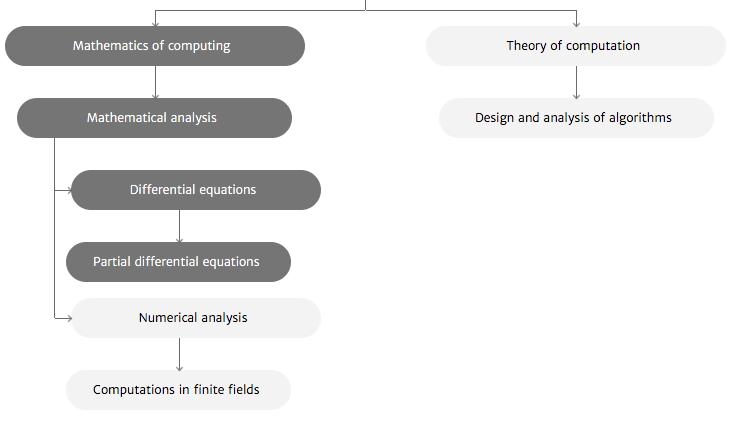
\includegraphics[width=\columnwidth]{figures/index.png}
   \caption{Conceptual location of the research project.}
\end{figure}

\subsection{A Note On The Word \textit{Linear}}
A non-linearity is essentially a characteristic that prevents a linear separation.

Despite the apparent linear character in algebra of the target equation, it is actually non-linear.
The introduction of the time variable~$t$~in the shape of the domain changes the operators at each time step during the integration procedure. 
Additionally, since the domain geometry will depend in some parameter values too, one cannot explicitly split the domain.  

Another type of non-linearity would be a term whose value depended on the field function $u$. 
These kind of non-linearities are common in mathematical modelling, but 




\section{Objectives and goals}
The research objective is to build a reduced order model for a parametrized heat diffusion problem with a moving boundary, 
by providing a concise description of the reducing procedure, 
a posteriori error estimators to certify their use and 
a use case to showcase computational costs and implementation details. 

Both the main equation of the PDE and the geometrical definition of the moving boundary are parametrized. 

\subsection{Scope}
A non-linearity is essentially a characteristic of a problem that prevents a linear separation.
Despite the apparent linear character of the naive heat equation, it is actually non-linear, since the introduction of the time variable $t$ in the domain changes the operators at each step. 

Another type of non-linearity would be a term whose value depended on the field function $u$. 
These kind of non-linearities are common in mathematical modelling, but 

We shall limit our research to this kind of problem, without the introduction of further non-lineariti

The project is mainly practice-oriented, in that we shall design, build and evaluate the procedure to construct the ROM.
Many reduction tools and strategies are available nowadays, each of them with their benefits and drawbacks. 



we intend to have theoretical content too.

By introducing the construction of a posteriori error estimators\footnote{Which rely on the usual stability factors and arguments present in Finite Element techniques.}, one can certify the results of the reduced basis for unseen in the training phase parameters.

%% Theory-oriented
% Theory development
% Theory testing

%% Practice-oriented: intervention cycle
% Problem Analysis
% Diagnosis
% Design
% Change
% Evaluation


%% Research Strategy
% Suitability
% Duration
% Feasibility



\newpage
\section{Conclusions}
\label{sec:conclusions}

\printbibliography

% http://danceswithcode.net/engineeringnotes/rotations_in_3d/rotations_in_3d_part1.html

\end{document}




\newpage
\printbibliography

\end{document}